% #############################################################################
% This is Chapter 3
% !TEX root = ../main.tex
% #############################################################################
% Change the Name of the Chapter i the following line
\fancychapter{Localization}
\cleardoublepage
% The following line allows to ref this chapter
\label{chap:architecture}

This chapter explores in detail the comparison between different packages to solve the localization problem. We test three packages, each one using a different approach.
To evaluate the accuracy of each package, we used a provided python script, which computes the difference between the ground truth robot position and the estimated one. This script was adapted to compute the average position error.
% #############################################################################
\section{Ground Truth}

The ground truth is an important piece of data that will let us compare our position estimates with the real robot position in the future. Looking at the github repository where we got the dataset from, it is said the following: `The ground-truth data is provided in the /tf topic, as a transform \(mocap \rightarrow \mathrm{mocap\_laser\_link}\)`.

In order to be able to view the evolution of the ground truth on the map, a script was created. This script, listens to the transformations \(mocap \rightarrow \mathrm{mocap\_laser\_link}\) being published on the /tf topic, retrieves its translation and rotation from the mocap frame and accumulates them on a list. Due to that, it creates a list with all the robot previous positions. It then publishes this list of points on a new topic. Having done so, we can now easily run rviz and add a path that listens to the topic where the accumulated positions are being published. The result of the previous actions can be visualised in the figure ...., where the thin green line represents the real robot path.

\begin{figure}[h]
\centering
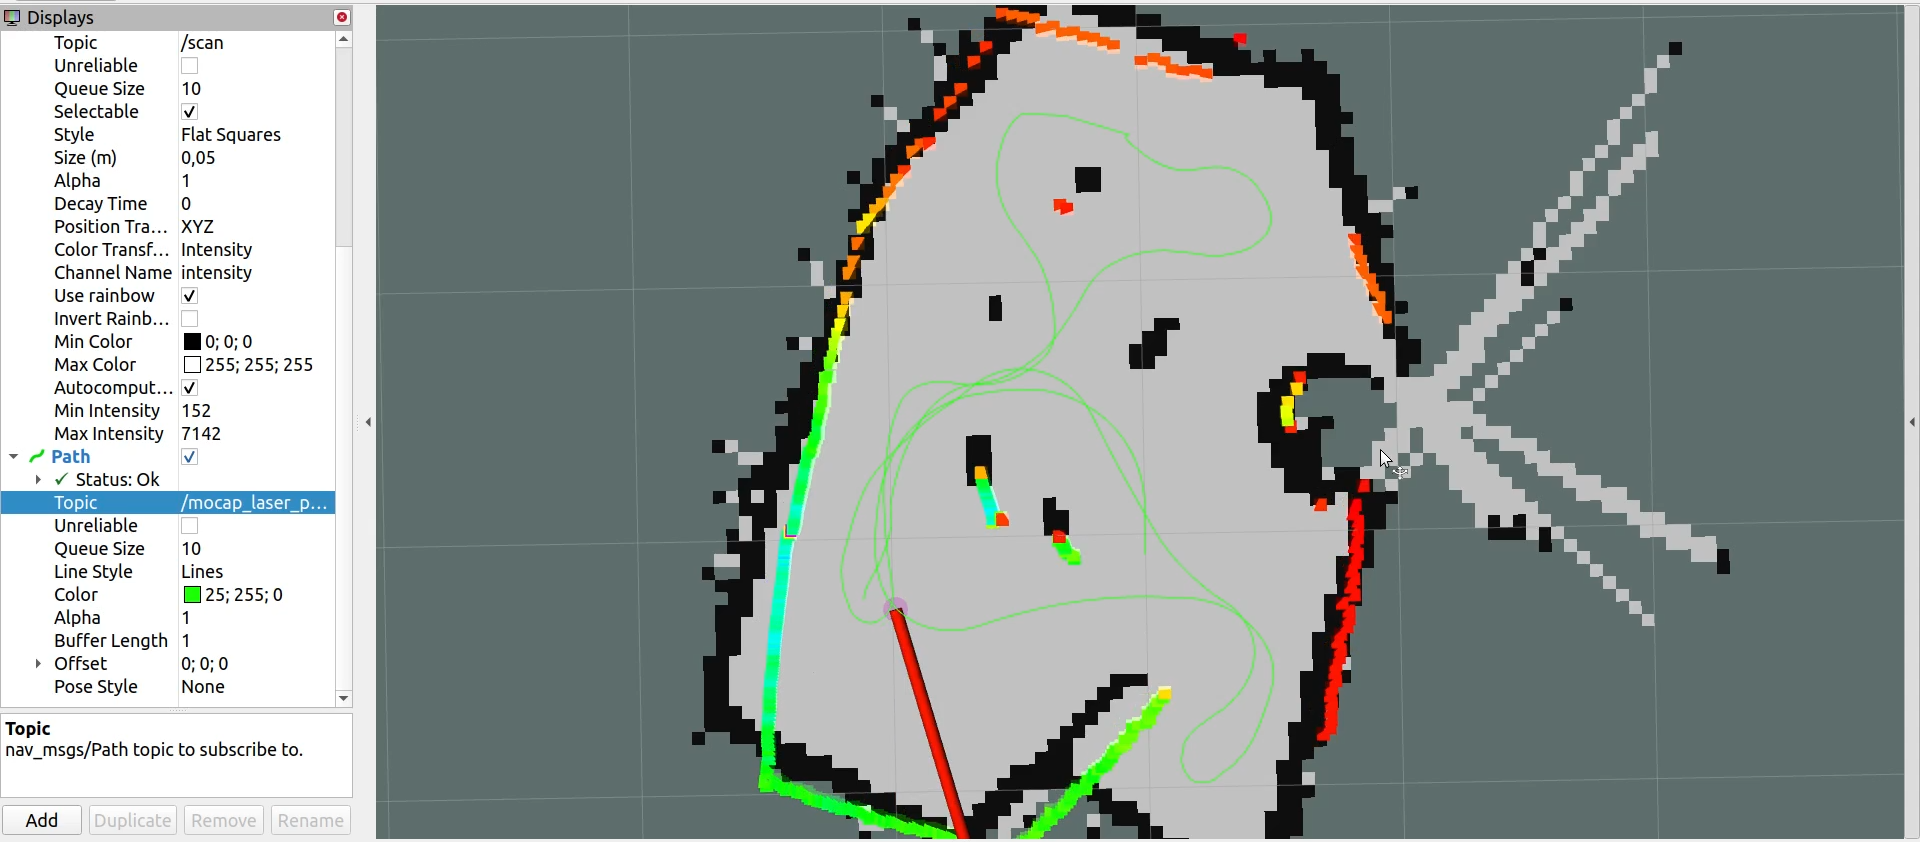
\includegraphics[scale=0.2]{./Images/mocapRviz}
\caption{Robot ground truth path}
\label{fig:flowchart}
\end{figure}

\section{Robot Localization Package}

In this section we will walk you through our progress using the robot localization package, in conjunction with the Extended Karmen Filter algorithm. 

Our first interactions with the ekf algorithm did not go too well. There was a consistent problem of having the robot estimate position outside the map, which can be observed in the figure ....

\begin{figure}[h]
\centering
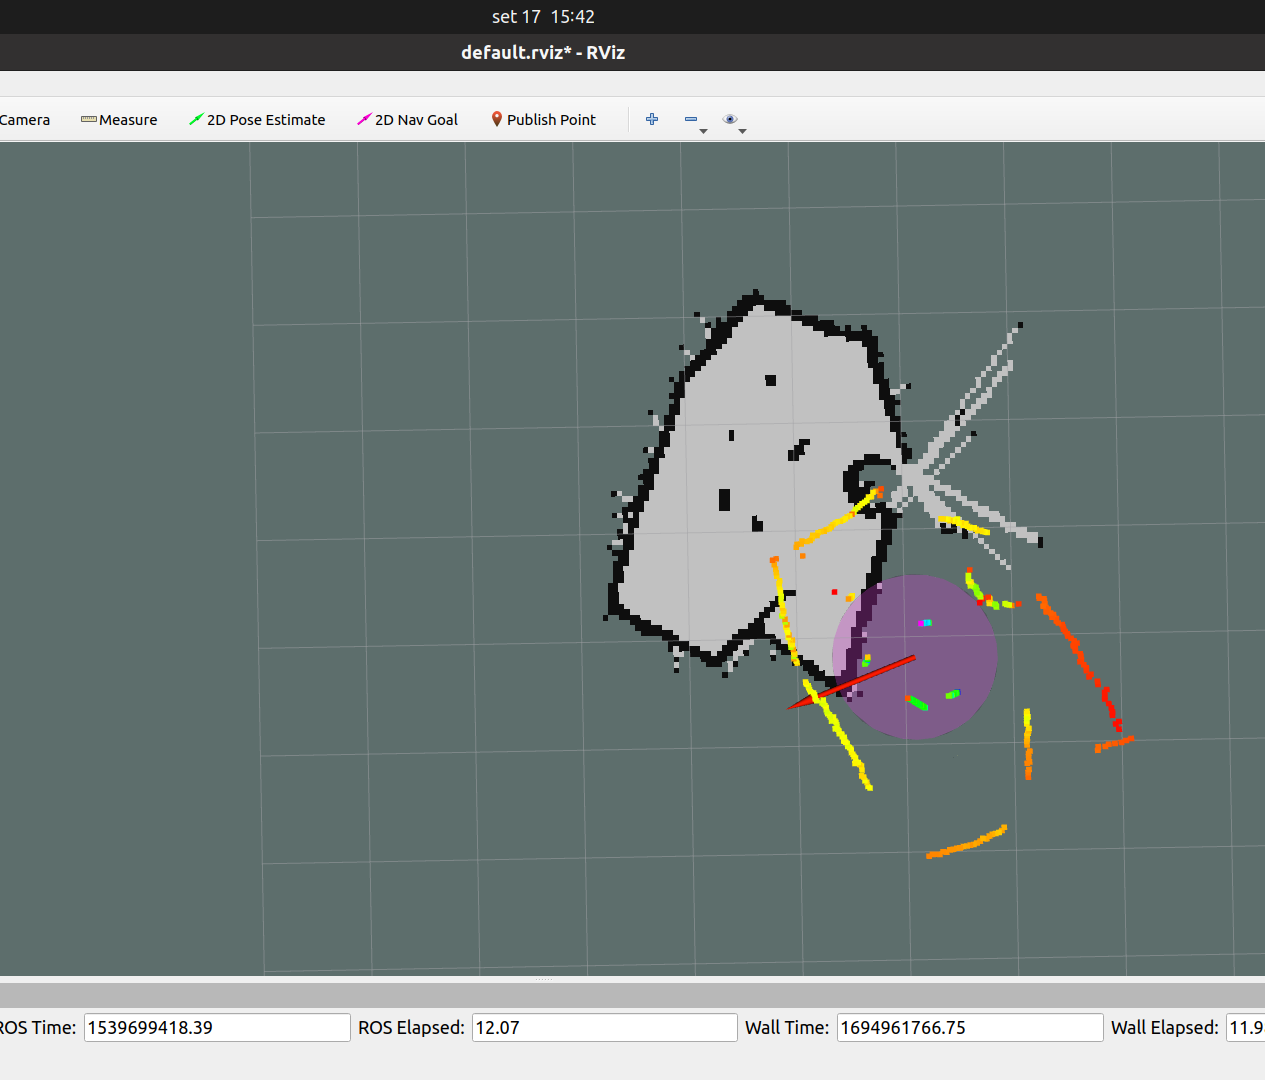
\includegraphics[scale=0.4]{./Images/ekfOutsideMap}
\caption{Using ekf algorithm on the dataset provided map}
\label{fig:flowchart}
\end{figure}

The solution, at first, to this problem was found in the parameters of the robot localization package. There is one particular parameter called "publish\_tf" which when set to false, solved the problem of the laser being readings being outside the map. It also made the error between the robot true position (ground truth) and the robot estimate position, represented by the "base\_scan" frame, smaller than when using the parameter set to true. 

\begin{figure}[h]
\centering
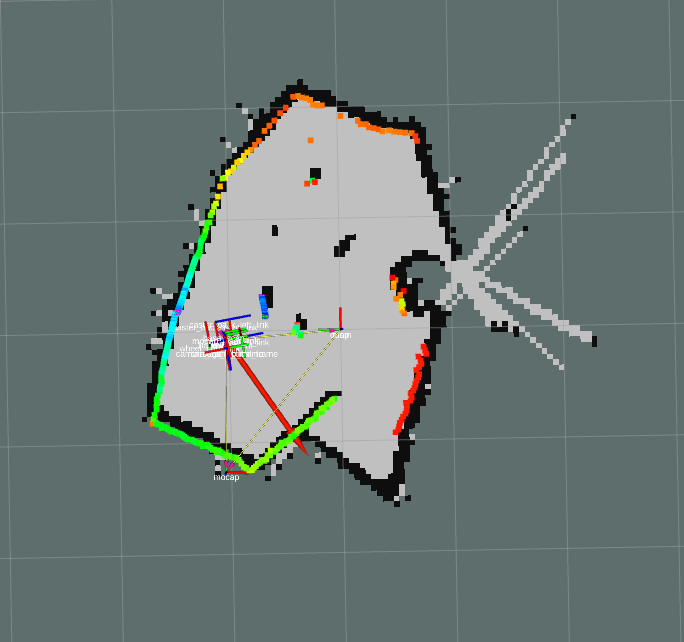
\includegraphics[scale=0.5]{./Images/tfPublishFalse}
\caption{Using the "publish\_tf" parameter set to false}
\label{fig:flowchart}
\end{figure}

Unfortunately, we later found that this could not be the solution to our problem. If we observe the list of topics being published, two of them are relevant to this problem: "/odom" and "/odometry/filtered". They both represent odometry values but their difference is that, while the first one publishes odometry raw data comming from the robot wheel's enconders, the other is the result of using the ekf algorithm with the fused data from the odometry and the imu. In other words, the "/odometry/filtered" topic publishes the position estimated by applying the ekf algorithm, which is what we truly want to test. Returning to the previous solution found, when we set the "publish\_tf" to false, the "base\_scan" frame will represent the raw data from /odom and not the estimated position from /odometry/filtered. Since that, we can not use this solution and must keep the "publish\_tf" parameter set to true.

We will know talk about the final config that we chose for the robot localization package. The parameters that we found more useful were:

\begin{itemize}
    \item Frequency: Increasing the frequency helped reducing the error. This is due to the fact that, since we are making estimates in smaller time intervals, the estimation error will be smaller because the robot traveled less space between estimates and so, it is less uncertain about his current position. Sadly, this technique has some drawbacks. When using greater frequency values some of the message can be lost, making so that when the script to calculate the error was run, it would give different results from run to run. For this reason and after some tests, the value 30 was chosen.
    \item Two D Mode: Since we are operating in an almost totally planar room, for simplicity we set this parameter to true.
    \item Frame: The frame parameters where set up in conformity with the official ros robot localization documentation.
    \item Sensor Config: 
        \begin{itemize}
            \item Odom: 
            \item Imu:
        \end{itemize}
    \item Process Noise Covariance:
    \item Publish Tf: As mentioned before this parameter was set to true.
\end{itemize}

\section{Results On Positioning By Different Algorithms} 

\begin{table}[htb]
\centering
\normalsize
{\footnotesize
    \caption{Position Error Results}
    \label{tab:streamingtech}
    \begin{tabular}{ | c | c | c | c |}
    \hline
    & Gmapping & EKF & AMCL\\
    \hline \hline

    Error (mm) & 37.04 & 64.11 & 43.54 \\
    %\textbf{Protocol} & & & \\ 
    \hline
    
    \end{tabular}
    }
\end{table} 

\section{Changed Parameters} 
\begin{itemize}
    \item imu0\_differential: For each of the sensor messages defined above that contain pose information, users can specify whether the pose variables should be integrated differentially. If a given value is set to true, then for a measurement at time t from the sensor in question, we first subtract the measurement at time t−1, and convert the resulting value to a velocity. This setting is especially useful if your robot has two sources of absolute pose information, e.g., yaw measurements from odometry and an IMU. In that case, if the variances on the input sources are not configured correctly, these measurements may get out of sync with one another and cause oscillations in the filter, but by integrating one or both of them differentially, we avoid this scenario. (EXPLICAR MELHOR ISTO)
\end{itemize}

\section{AMCL}
To estimate/obtain robot localization, it is also possible to use another package: AMCL. This package implements the adaptive (or KLD-sampling) Monte Carlo localization approach (as described by Dieter Fox), which uses a particle filter to track the pose of a robot against a known map. For this experimentation, we also used a recorded rosbag, capture from the IST LAB, using the Turtlebot\_3. The results were observed using the RVIZ programm.

\subsection{Main Principle}
This algorithm, at runtime, will start by spreading the particle number at the initial position (initial robot location estimate). Then, it makes a prediction of the robot location, based on the odometry (maybe IMU too?). Then, it compares the prediction with the laser scan (new mesurements), and updates the particles weights. Next, it resamples the particles, based on the weights, meaning it will discard the particles with lower weights, and will duplicate the particles with higher weights. It repeats the process over and over. 
Overall, with time, the particles will follow a possible robot location.

\subsection{Test Conditions And Expected Results}
For this test, the robot was teleoperated, in the LSD4 LAB, with the map in the image (REFERENCIAR IMAGEM), computed previously. The initial true position is x:0 and y:0. This means that if we already give the correct initial position, the number of particles will meet the true robot position, and the algorithm will quickly converge to the true robot position.
Yet, to test how the number of particles affect this algorithm, we first start to change the initial position to other values, away from the original one. Only after that, we changed the particle number, to try to compensate for the bad initial position.

One important note is that the Ground Thruth is not availbale, and so, the only option to acess how effective the algorithm is progressing, is to observe the estimated path in the RVIZ. (TALVEZ TENTAR ARRANJAR UMA FORMA MELHOR DE PRODUZIR RESULTADOS!)


\begin{figure}[h]
\centering
\vspace{3pt}
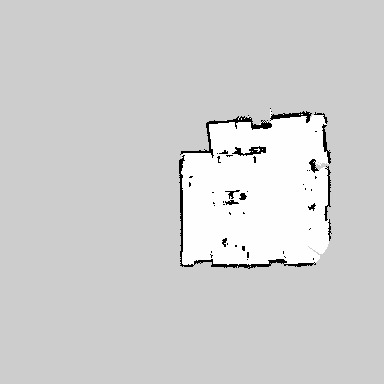
\includegraphics[scale=0.4]{./Images/2023-09-18-10-18-29}
\caption{LSDC4 room map}
\label{fig:flowchart}
\end{figure}


\subsection{Tuning Parameters}
At the moment of writing, the only parameters changed were the MIN and MAX number of particles. We are assuming the number of particles, at runtime, might change between the MIN and MAX set. For instance, if the algorithm is very sure of its estimate, it reduces the particles number. Otherwise, it might increase the particle number. This was not yet confirmed by trustable sources (CONFIRMAR ISTO / TALVEZ NEM SEJA IMPORTANTE).

At first, we started with a conservative number of particles, with particles between 500 and 3000, being the AMCL ROS package default value. We also set the initial algorithm estimate to the true position. The results show that the estimated position seem correct, since the laser readings match the map boundaries \ref{fig:amcl-lab-rosbag-0-0-500-3000}.
\begin{figure}
    \centering
    \includegraphics[width=1\linewidth]{Images/amcl-lab-rosbag-0-0-500-3000.drawio.png}
   \caption{AMCL iteration, with correct initial position (x:0, y:0), and default number of particles ([500-3000])}
    \label{fig:amcl-lab-rosbag-0-0-500-3000}
\end{figure}

Then, we proceed to alter the initial AMCL position (but not the number of particles), a bit to the right. The results show that the AMCL tries to correct the estimated position, a bit to the left \ref{fig:amcl-lab-rosbag--1--1-500-3000}.

\begin{figure}
    \centering
    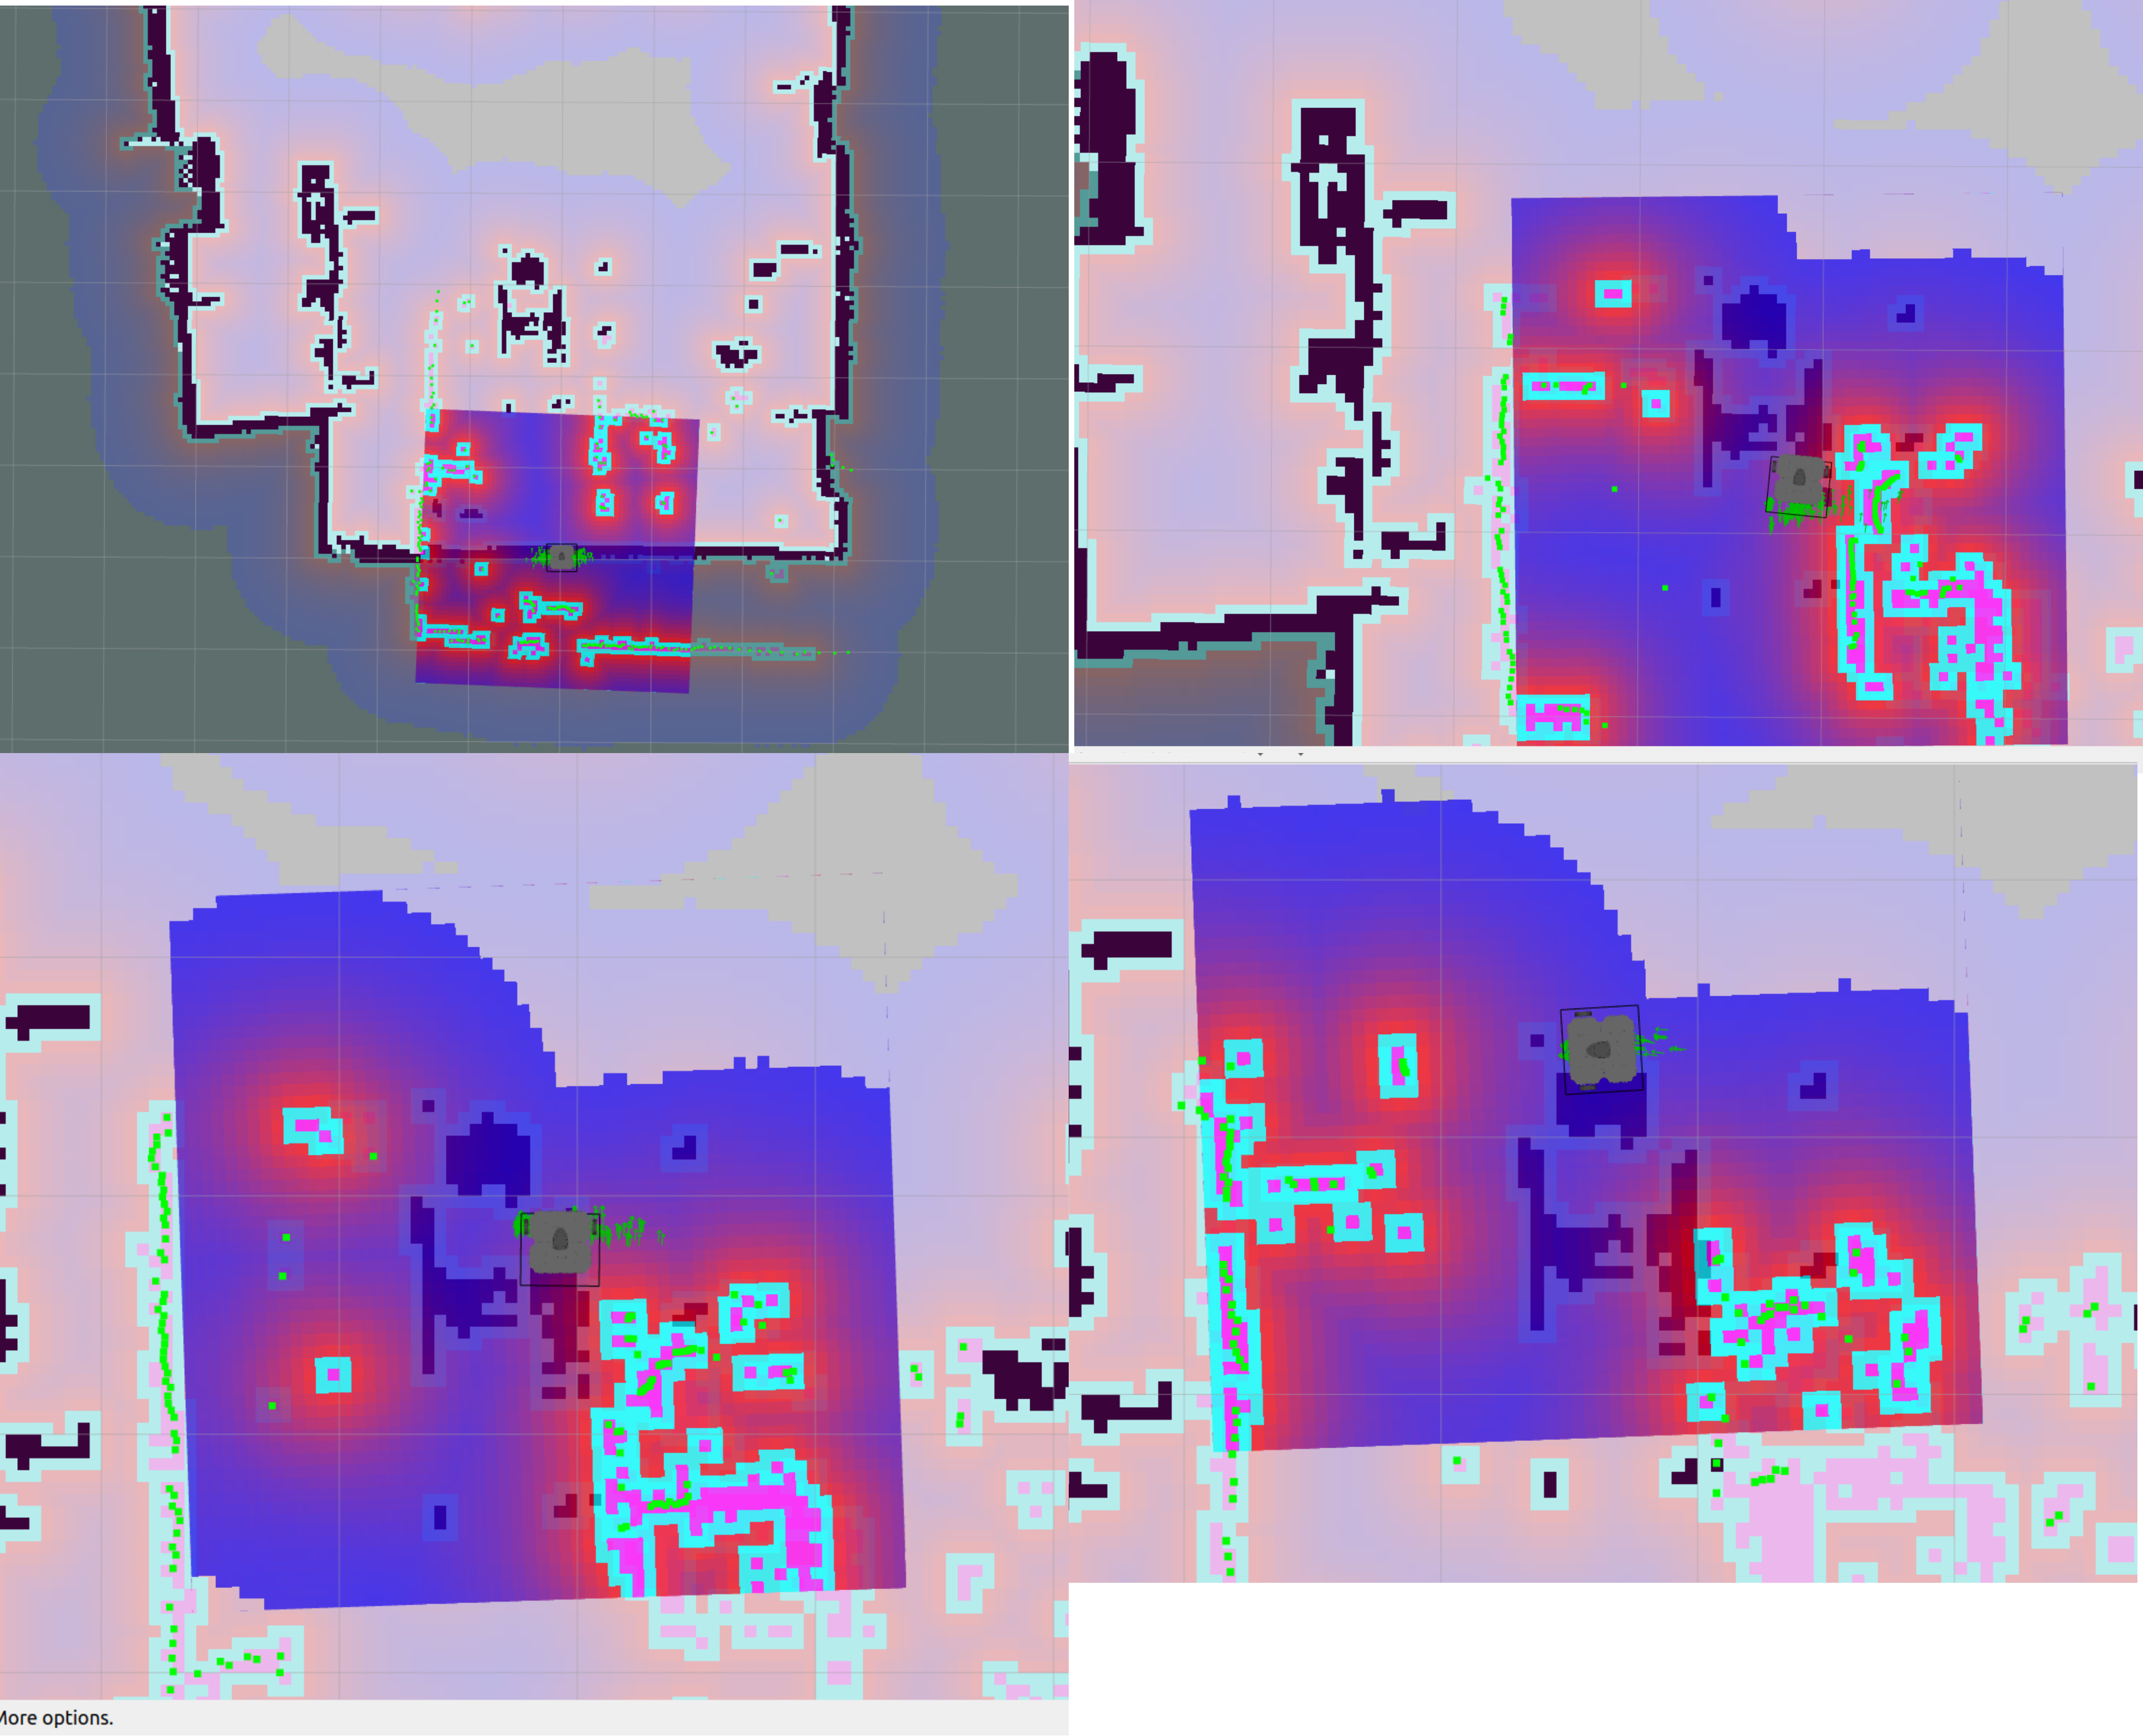
\includegraphics[width=1\linewidth]{AMCL iteration, (x -1, y -1)-([500-3000]).png}
    \caption{AMCL iteration, with wrong initial position (x:-1, y:-1), and default number of particles ([500-3000])}
    \label{fig:amcl-lab-rosbag--1--1-500-3000}
\end{figure}

Yet, this correct is not very noticeable. To allow for a better comparison, the particles were duplicated (from [500-3000] to [1000-6000]). The results show a big increase in the correction shift \ref{fig:amcl-lab-rosbag--1--1-1000-6000 - first iter}.

\begin{figure}
    \centering
    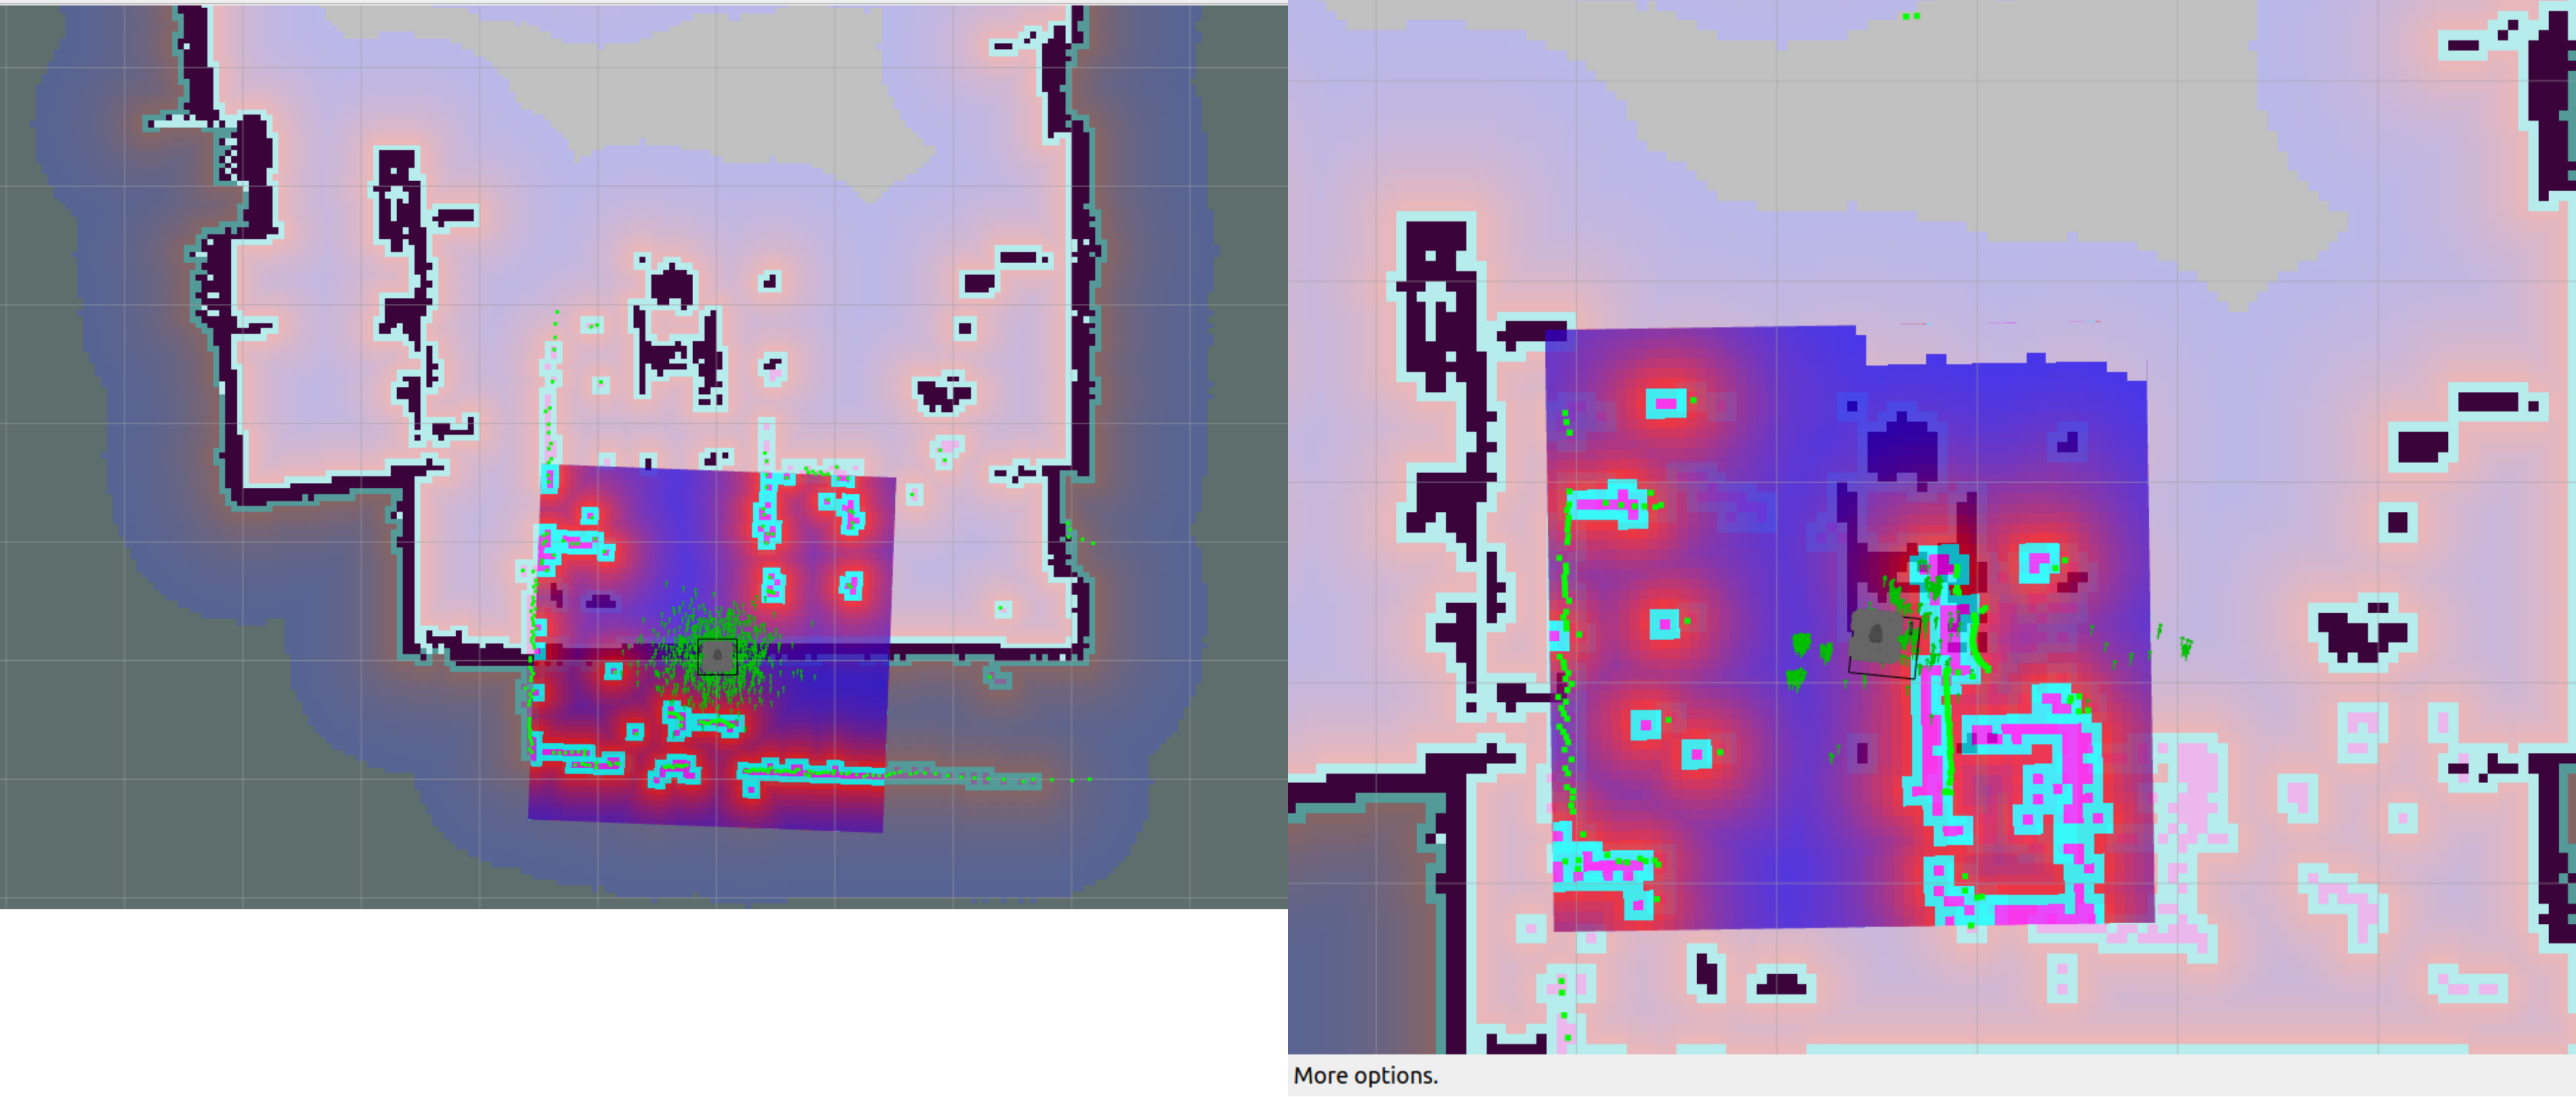
\includegraphics[width=1\linewidth]{AMCL iteration, (x -1, y -1)-([500-3000])(1).png}
    \caption{AMCL iteration, with wrong initial position (x:0, y:0), and default number of particles ([500-3000]) - First Iteration}
    \label{fig:amcl-lab-rosbag--1--1-1000-6000 - first iter}
\end{figure}

This means that the algorithm tends to converge to the correct position much faster when the number of particles is increased. This can be explained duo to the probability of existing particles in the right robot pose being much higher, which will then receive more weights, leading to a faster convergence.

Then, the same test was conducted, exacly with the same parameters as in the last paraghraph. The results continued to show a level of correction shift to the left, but not as accentuated as preveouly \ref{fig:amcl-lab-rosbag--1--1-1000-6000 - second iter}. 
This happens because when the AMCL algorithm starts, the initial destribution of particles is random. In the first iteration, by pure chance, the particle destribution was probably closer to the true robot's pose, leading to a better and faster correction. 

\begin{figure}
    \centering
    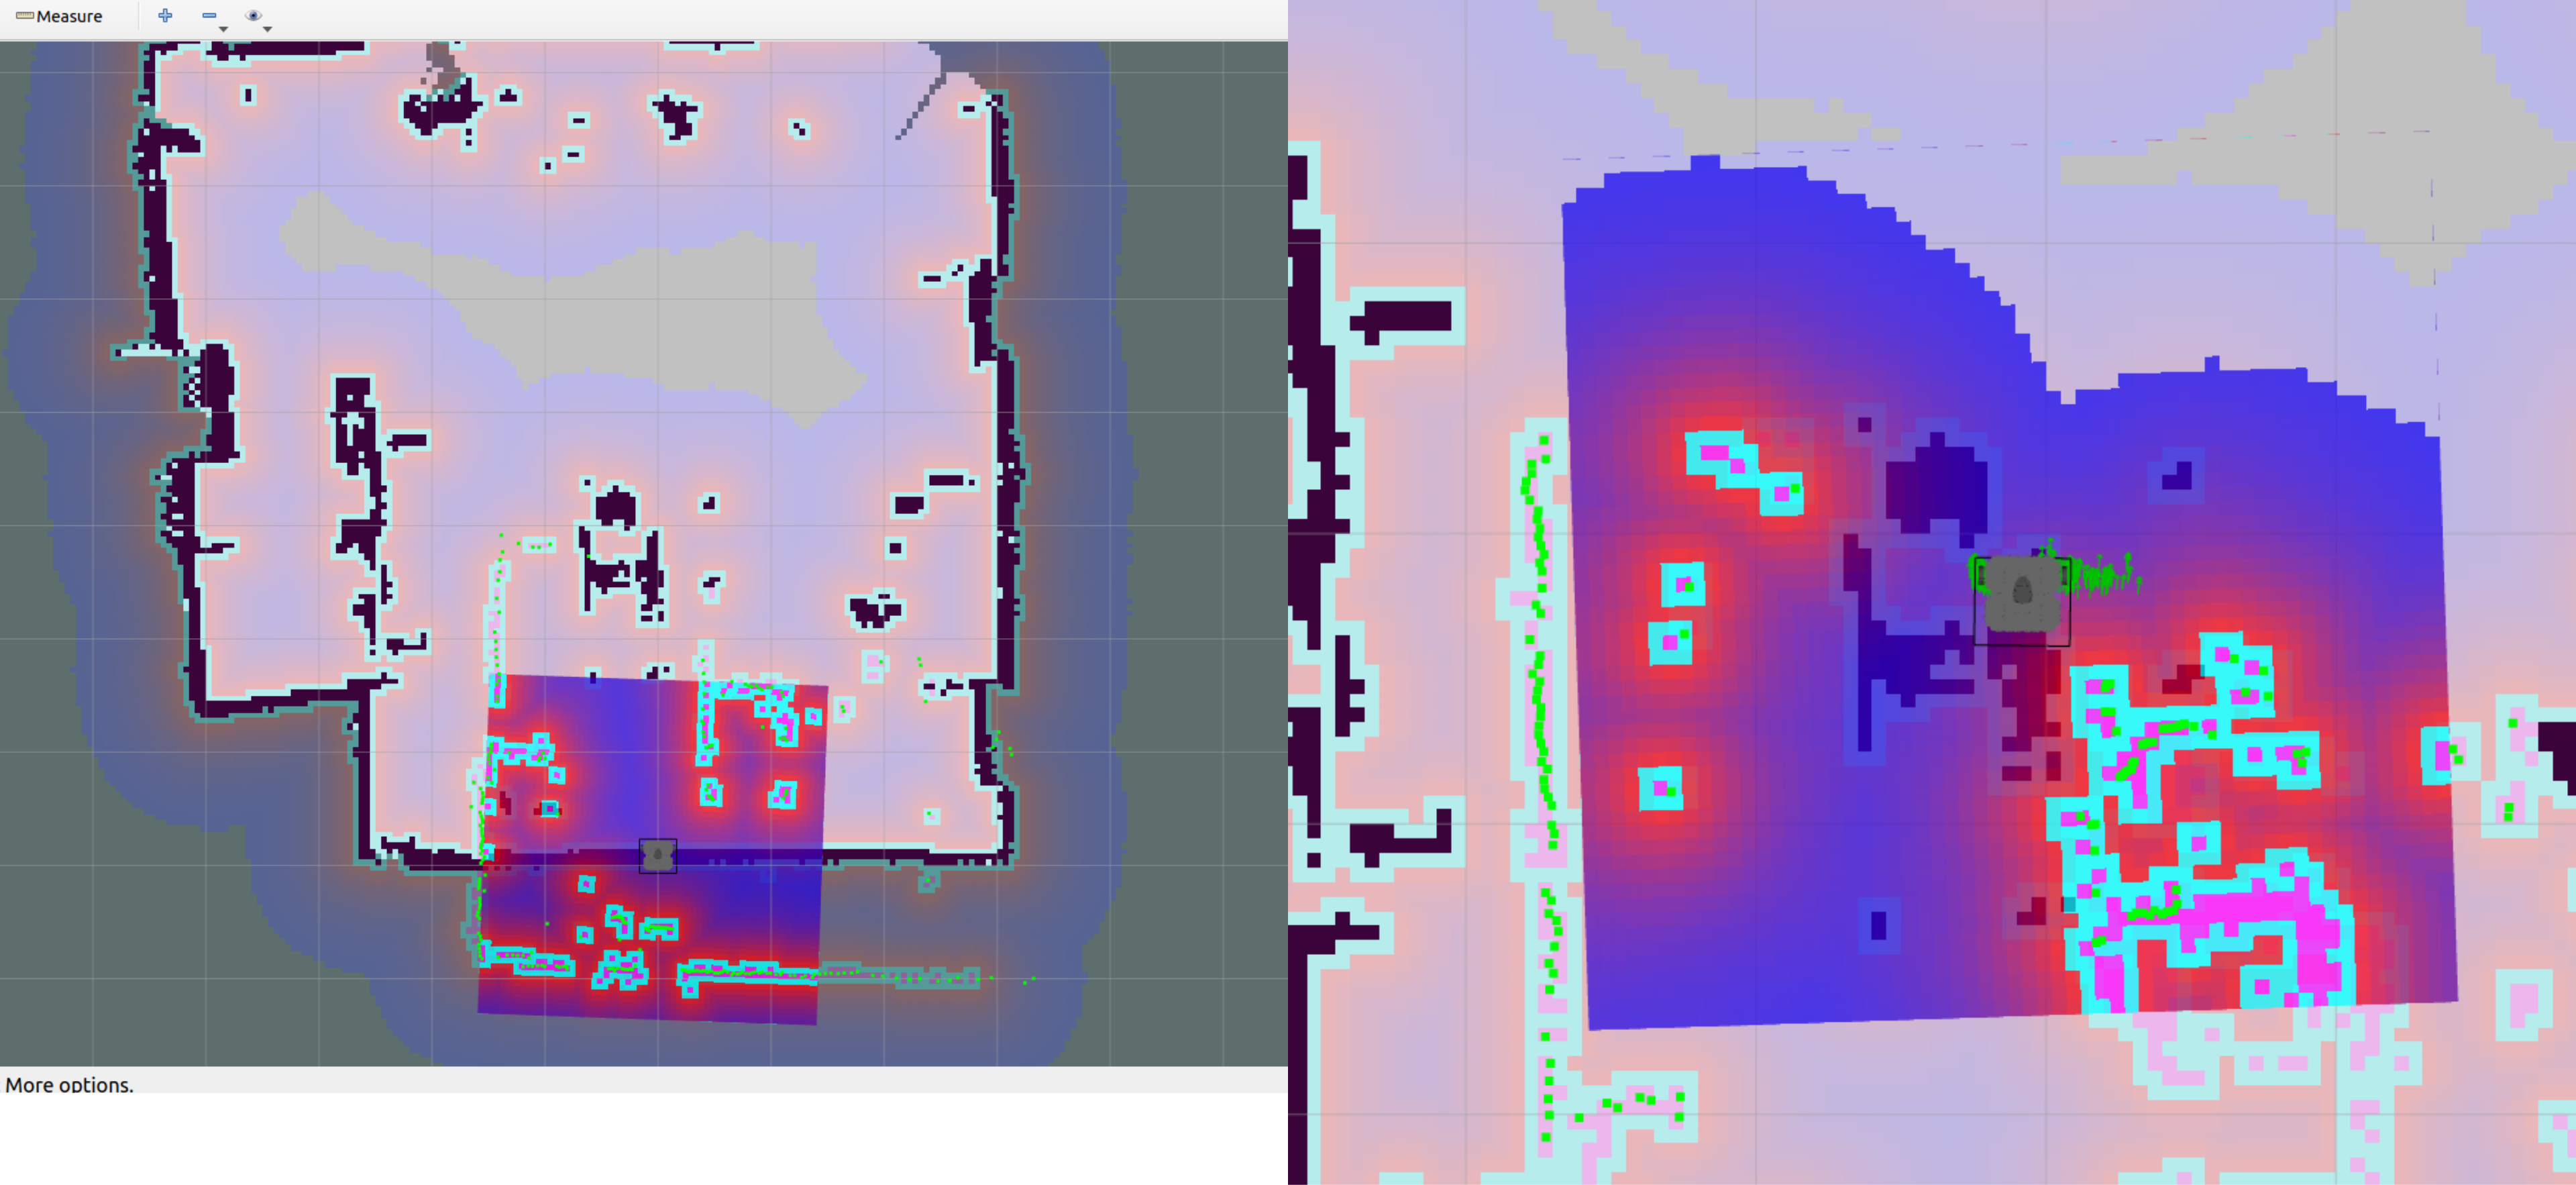
\includegraphics[width=1\linewidth]{amcl-lab-rosbag--1--1-1000-6000.png}
    \caption{AMCL iteration, with wrong initial position (x:0, y:0), and default number of particles ([500-3000]) - Second Iteration}
    \label{fig:amcl-lab-rosbag--1--1-1000-6000 - second iter}
\end{figure}

Finally, and to confirm the effect of the number of particles in the algorithm's performance, this one was lowered to just one particle, \ref{fig:amcl-lab-rosbag--1--1-1-1}. The results showed that no or little correction was made. This can be explained since one particle is not enough to explore the "environment" and thus, the probability of matching the real pose, when the robot receives new sensor measurements, is very low. 

\begin{figure}
    \centering
    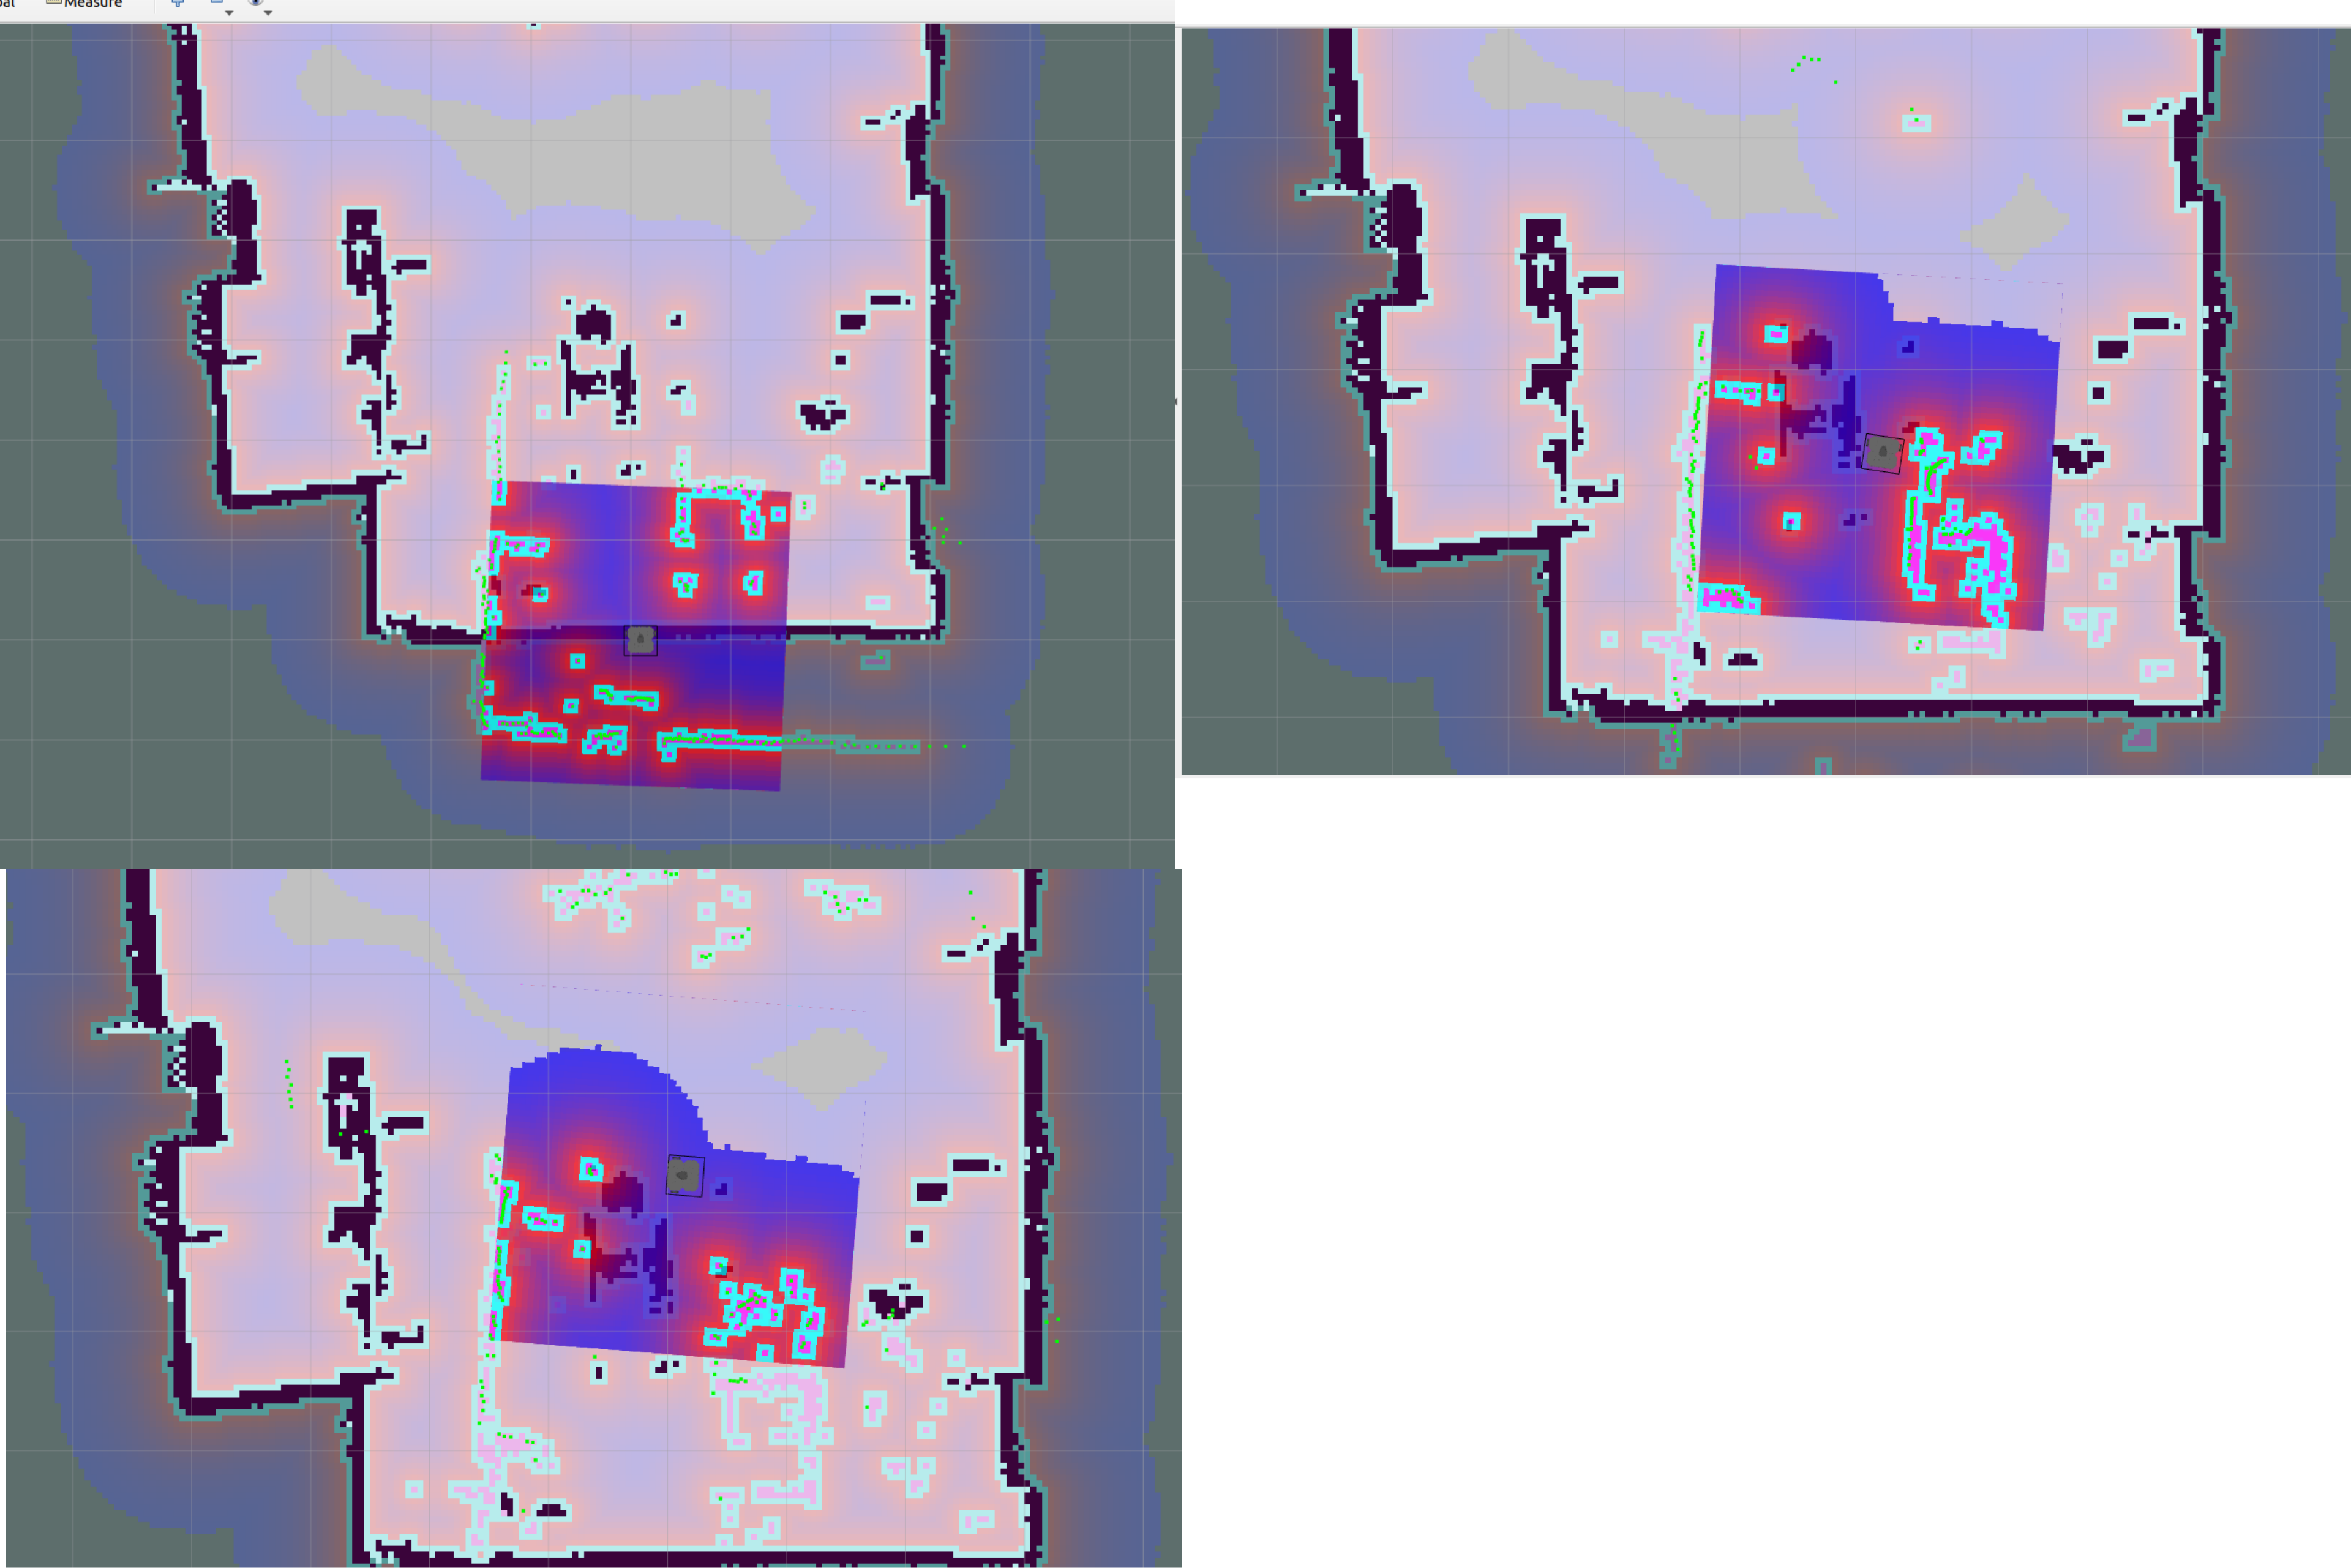
\includegraphics[width=1\linewidth]{amcl-lab-rosbag--1--1-1-1.png}
        \caption{AMCL iteration, with wrong initial position (x:0, y:0), and default number of particles ([1-1])}
    \label{fig:amcl-lab-rosbag--1--1-1-1}
\end{figure}

Now, lets see something interesting... Instead of placing the AMCL initial position shifted to the right, the initial position will be shifted to the left: (x:1, y:1). The number of particles stays the same as the default value: [500-3000]. The results \ref{fig:amcl-lab-rosbag-1-1-500-3000} show that, instead of shifting the robot's position to the right, in order to correct the initial right shifted position, the AMCL is actually shifting the robot to the left. Even when the number of particles is actually raised to 30000, the same thing happens most of the time \ref{fig:amcl-lab-rosbag-1-1-30000-30000}. {AINDA NAO SEI EXPLICAR ISTO}. If the number of particles is raised, the AMCL will use more data from new sensorial measurement to correct the estimated pose. If the corrections are being made in the oposite direction, this means that the particles are matching the wrong sensor mesurements. {SERA ESTA A CAUSA???}

Yet, this doesn't happen if the number of particles is again set to 1 (minimum value) \ref{fig:amcl-lab-rosbag-1-1-1-1}. The reason is because, since there is only one particle, the algorithm is going to use mostly the estimated pose, from the motion and not the measurement model. This explains why there is not left shift, as in the previous example.

\begin{figure}
    \centering
    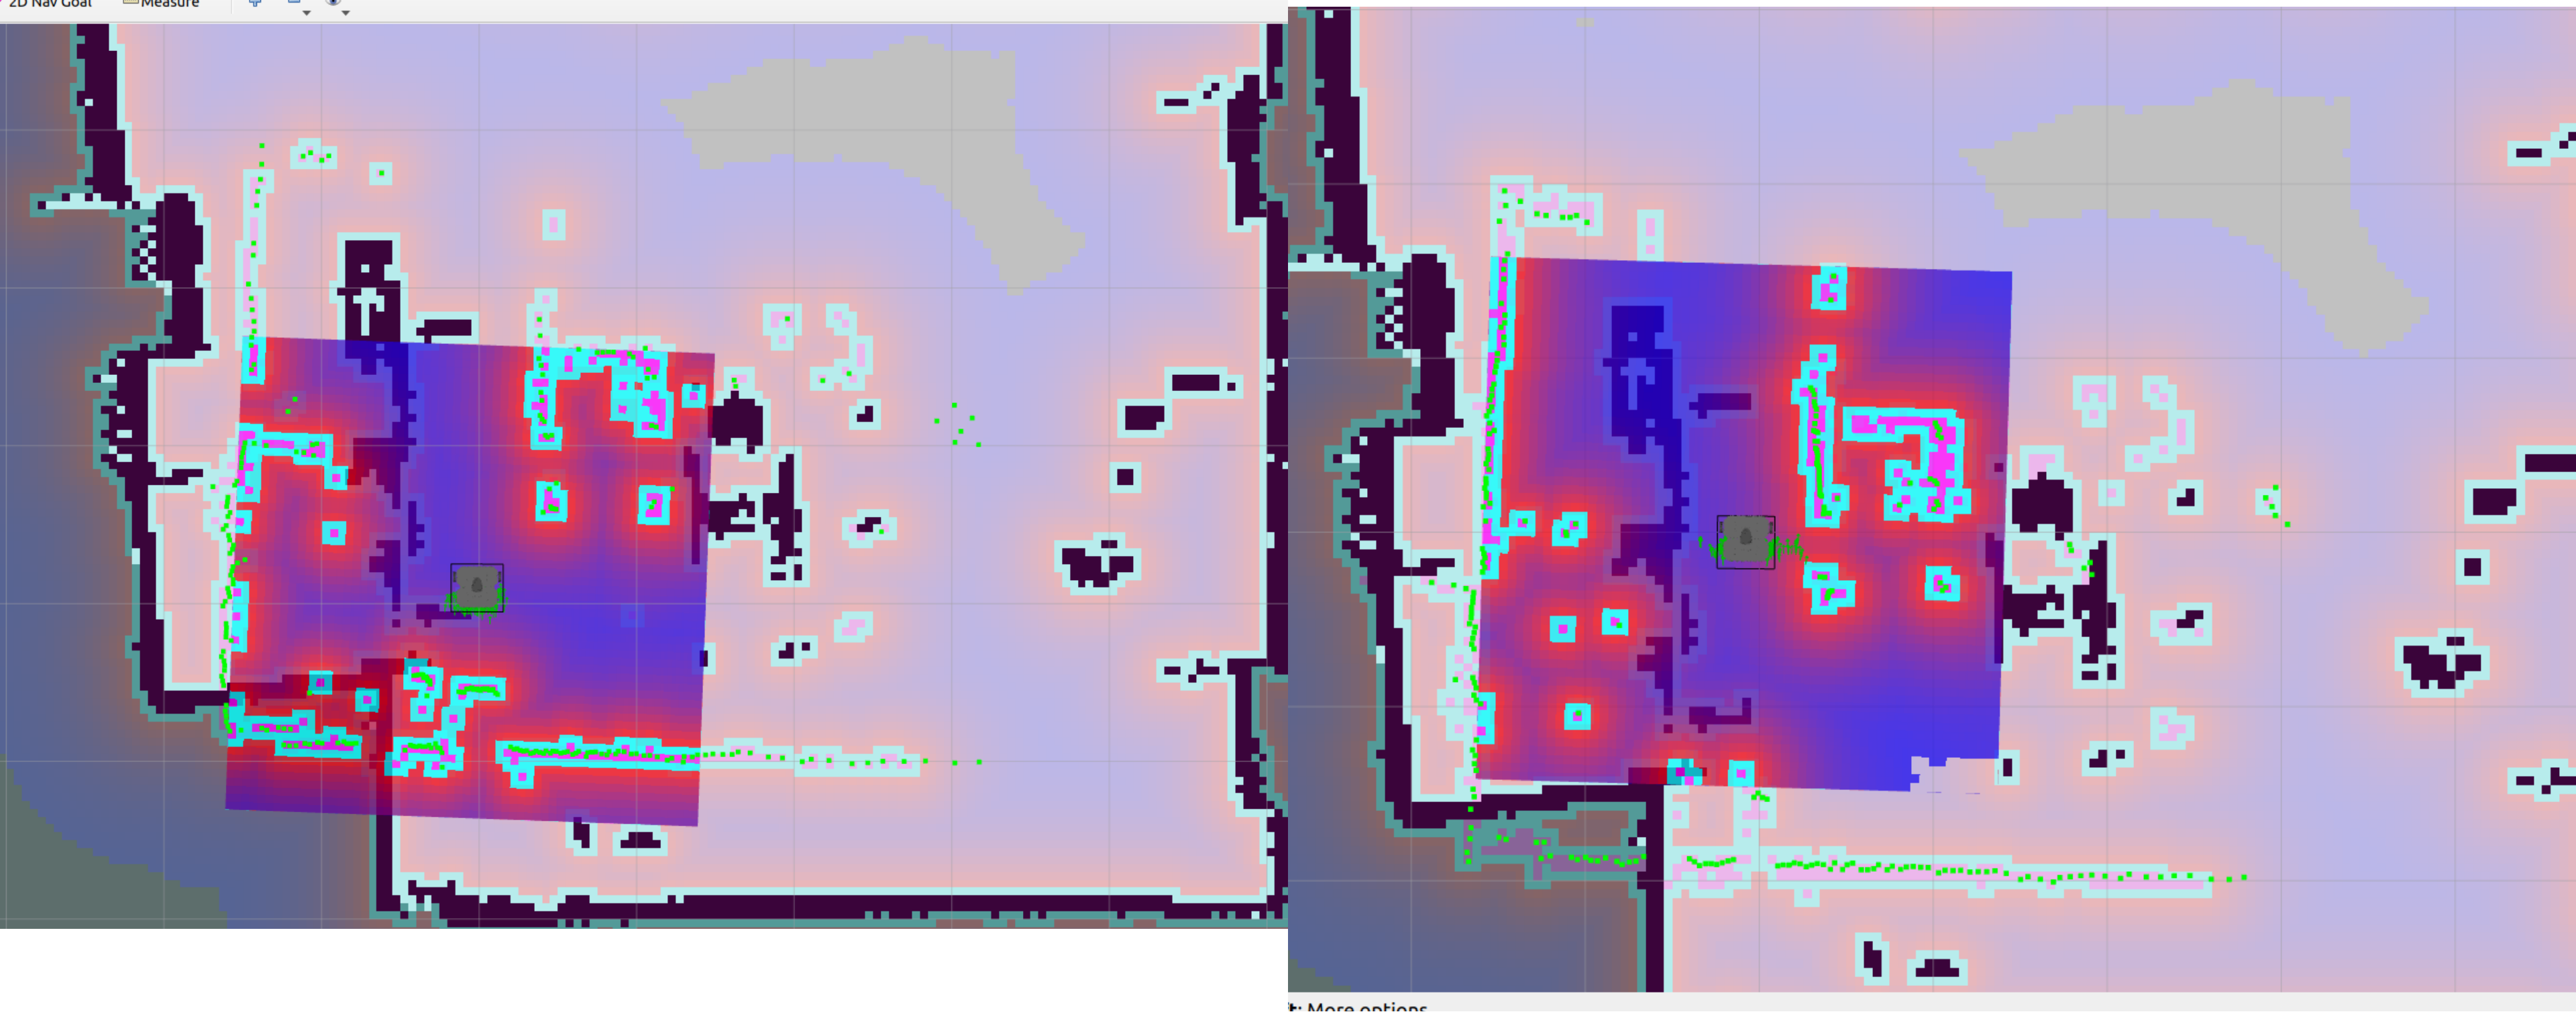
\includegraphics[width=1\linewidth]{amcl-lab-rosbag-1-1-500-3000.png}
    \caption{AMCL iteration, with wrong initial position (x:1, y:1), and default number of particles ([500-3000])}
    \label{fig:amcl-lab-rosbag-1-1-500-3000}
\end{figure}

\begin{figure}
    \centering
    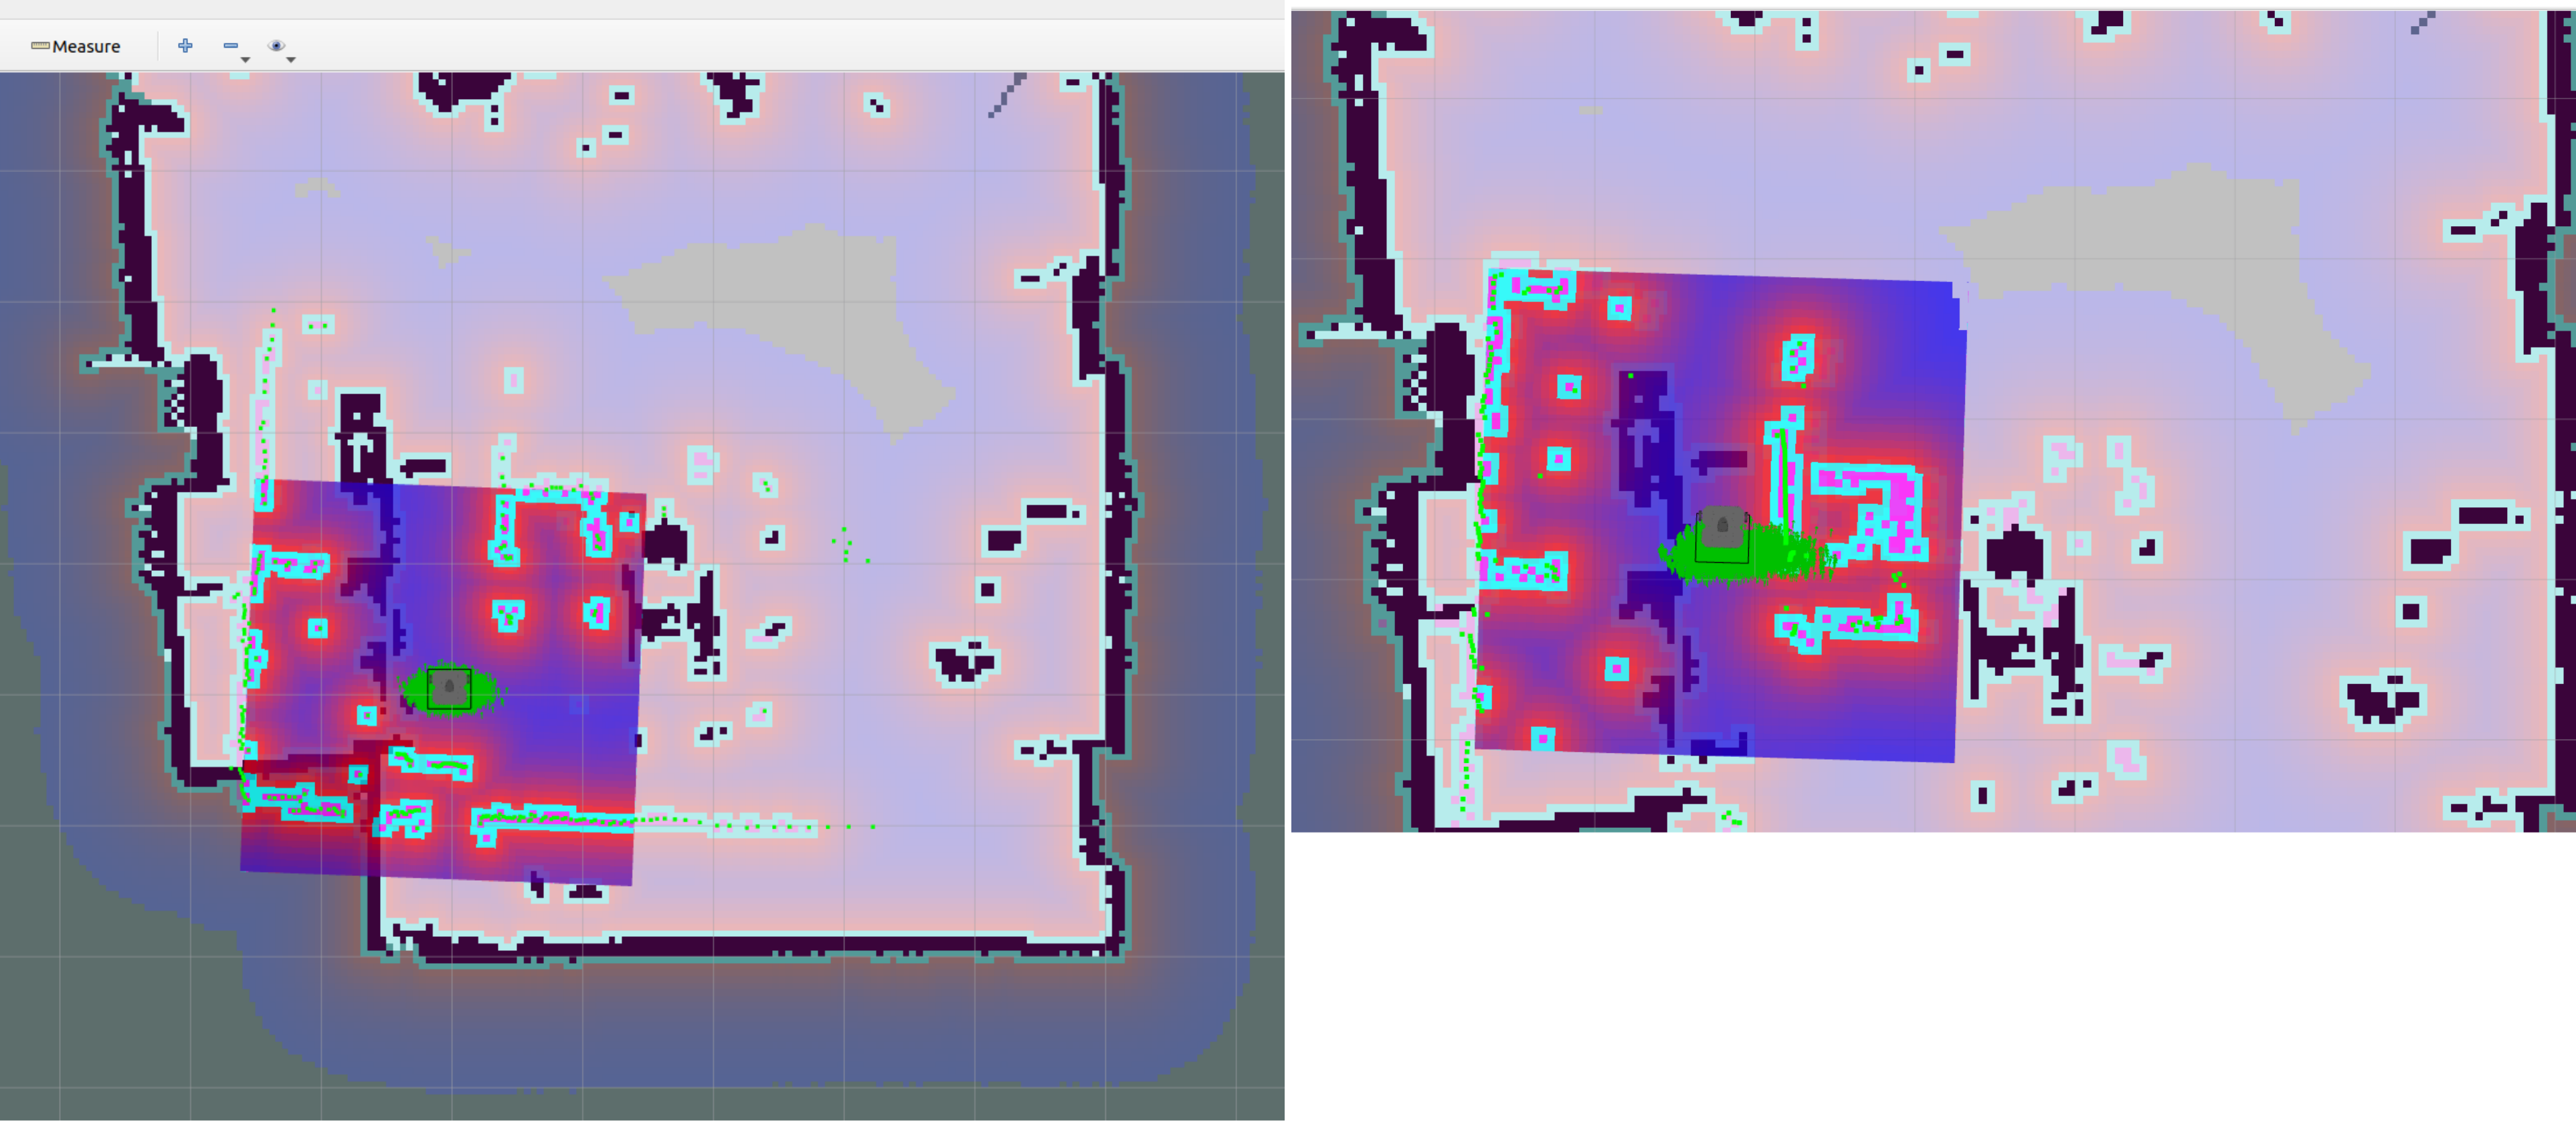
\includegraphics[width=1\linewidth]{amcl-lab-rosbag-1-1-30000-30000.png}
    \caption{AMCL iteration, with wrong initial position (x:1, y:1), and default number of particles ([30000-30000])}
    \label{fig:amcl-lab-rosbag-1-1-30000-30000}
\end{figure}

\begin{figure}
    \centering
    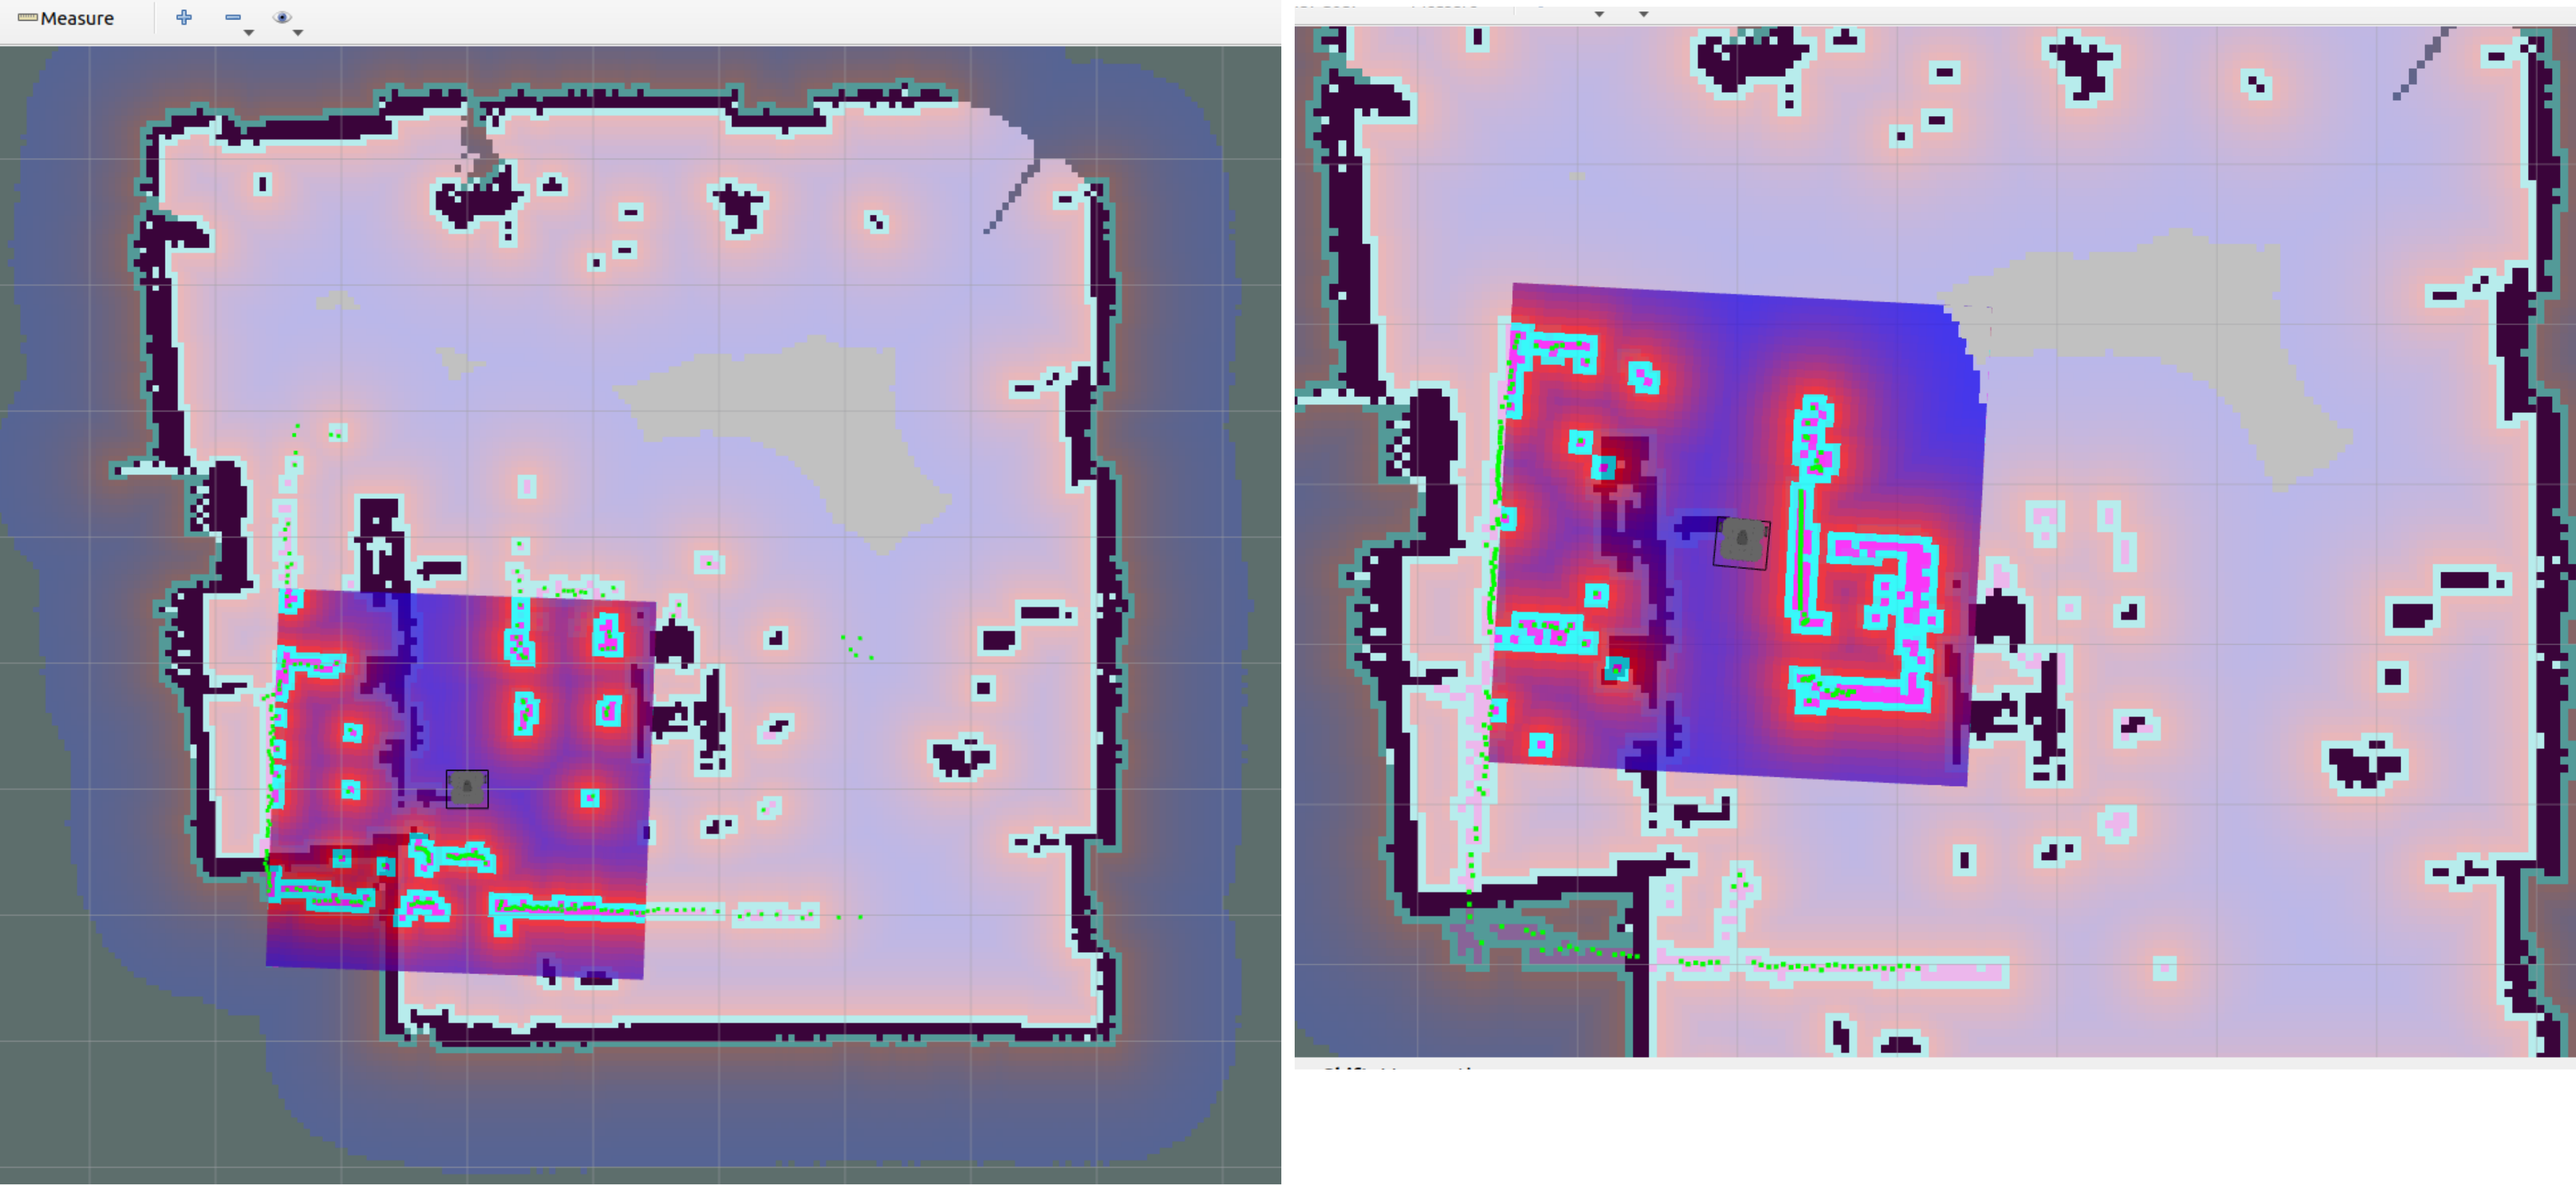
\includegraphics[width=1\linewidth]{amcl-lab-rosbag-1-1-1-1.png}
    \caption{AMCL iteration, with wrong initial position (x:1, y:1), and default number of particles ([1-1])}
    \label{fig:amcl-lab-rosbag-1-1-1-1}
\end{figure}